%&pdflatex
\documentclass[a4paper]{report}
\usepackage[margin=1in]{geometry}
\usepackage[utf8]{inputenc}
\usepackage{graphicx, longtable,pdflscape}
\usepackage{adjustbox}
\graphicspath{~/Year4Uni/diss/dissfiles}
\graphicspath{"~/Year4Uni/Dissertation/App screenshots"}
\usepackage{setspace}
\usepackage{float}
\usepackage{url}
\usepackage{listings}
\usepackage{color}

\definecolor{dkgreen}{rgb}{0,0.6,0}
\definecolor{gray}{rgb}{0.5,0.5,0.5}
\definecolor{mauve}{rgb}{0.58,0,0.82}

\lstset{frame=tb,
	language=Java,
	aboveskip=3mm,
	belowskip=3mm,
	showstringspaces=false,
	columns=flexible,
	basicstyle={\small\ttfamily},
	numbers=none,
	numberstyle=\tiny\color{gray},
	keywordstyle=\color{blue},
	commentstyle=\color{dkgreen},
	stringstyle=\color{mauve},
	breaklines=true,
	breakatwhitespace=true,
	tabsize=3
}

\doublespacing


\begin{document}

\title{
{Final Year Dissertation}\\ {Personal Safety Applications\\}}
\author{Jamie McCulloch\\Heriot Watt University\\H00189648\\jm7@hw.ac.uk\\MEng Software Engineering\\\\Supervisor: Mike Just\\\\Second Reader: Sven-Bodo Scholz}
\begin{figure}

\includegraphics[width=50mm, scale = 0.5]{logo.png}
\centering
\end{figure}
\date{}
\maketitle
\thispagestyle{empty}
\newpage
\begin{quote}
I, Jamie McCulloch, confirm that this work submitted for assessment is my own and is expressed in my own words. Any uses made within it of the works of other
authors in any form (e.g., ideas, equations, gs, text, tables, programs) are properly acknowledged at any point of their use. A list of references
employed is included.
\\ \\
Signed: 
Date: 
\thispagestyle{empty}
\end{quote}
\newpage
\begin{abstract}
As smartphone ownership continues to rise, they have become an integral part of society. Their capabilities and services are used daily, and continue to grow. The ability to track locations, contact relatives and emergency services within seconds, and instantly record video and audio has ensured that the general public can use their smartphones to improve their personal safety. However, this avenue has not been well explored, and question mark resides over this - are smartphones able to improve personal safety? 
\thispagestyle{empty}
\end{abstract}
\newpage
\tableofcontents
\thispagestyle{empty}
\newpage
\clearpage
\chapter{Introduction}
\label{sec:Intro}
\section{Overview}
\label{sec:Overview}
  Smartphone ownership is at an all time high, and it is imperitive that they are used to their full potential. With this in mind, one area in which there is not a lot of research or evaluation into is personal safety. Smartphones are able to do many things, such as:
\begin{itemize}
    \item track GPS location
    \item store thousands of contacts
    \item record video and audio instantly
    \item access the internet through broadband cellular networks
  \end{itemize}
 It is now possible for people's location to be tracked, for others to be immediately contacted, and instant proof of crime
  through video/audio recording. The rise of social networking has allowed people to spread news, and their own personal experiences of certain areas within their local community,
  allowing people to gauge what surrounding areas are safe to walk or not.
   \section{Aims and Objectives}
   \label{sec:AimsAndObj}
    The aim of this project is to develop a smartphone application that improves the personal safety of its user while they are walking outside alone. This will be done through location updates and tracking, an emergency panic button, alternate route planner, among others. The objectives for this project are listed below:
    \\ 
    \begin{itemize}
    	\item \textbf{Designing the application}
    	\\
    Designing a personal safety application with an intuitive user interface, that users can easily follow and complete tasks with, and with features that people want. I have carried out an online survey, with 74 participants, asking their opinion of personal safety applications and if they would find them useful. The survey comprised of 9 questions, and a copy of the survey questions is available in Appendix A. I kept the survey online for 5 days, then closed it and sorted through the responses. I also used the survey to gather requirements for the application laid out in section \ref{sec:Requirements} of this document. I intend to create use cases during the design stage of the project, as well as designing the user interface, and the prototypes for this project. 
    \\ \item \textbf{Building the application}\\
	I have implemented my own personal safety application, using the research I've found.  I implemented features from other applications (panic button, alarm button, location tracker) but also intended
	some of my own ideas (a journey countdown timer, a proximity based social media, time filters). I created three prototypes, laid out in section \ref{sec:Imp}, with incremental differences, resulting in a fully functional application that implements the most popular features laid out in section \ref{sec:FunctionalReq} of this report, as well as a few others. 
    \\ \item \textbf{Evaluating the application}\\
    Once I created a prototype application, I then recruited a small group of participants and conducted an interview with them to get their feedback in terms of the application. I asked them to complete tasks on the application, and asked if they have any improvements they would make. More information on the usability study is found in section \ref{sec:Usability} of this report. 
\end{itemize}
\section{Challenges and Possible Solutions}
\label{sec:ChallengesAndSolutions}
  The challenge with personal safety applications is how people determine somewhere being unsafe. For example, social media can be used to alert to unsafe locations, or unusual activity, but with the sheer scale of information on social media, and the privacy surrounding individual profiles, this information can easily get hidden or missed. The proximity based social media platform I hoped to integrate into my application may potentially solve this, as anyone will be able to post to it and only those in a certain area will be able to see posts.
  \\ There are many factors that determine
  if somewhere is unsafe - noise level, past crime rate, time of day, the people residing there, etc., \cite{mccarthy} and these all have to be considered individually and refined.\\
  People may not want to be able be tracked, or want to know when they are entering an unsafe location, essentially, due to privacy concerns  \\ \\
  I had hoped that my personal safety application would prevent these problems. It would extract information from local council/authority Facebook/Twitter feeds, and also rely on users
  contributing directly to the application, anonymously, their experiences. The application would run only when the user selects it, and all features are able to be turned off and on
  as the user pleases. While not in this implementation, in section \ref{sec:FuturePlans} I discuss future plans in terms of the application. 
\section{Layout of Dissertation}
\textbf{Section 2:} In this section I have conducted a literature review into the topic of personal safety, including differences in gender and age, problems with personal safety applications, and the need for a personal safety application, among others. \\
\textbf{Section 3:} Using my survey, I derived requirements, both functional and non functional, and conducted analysis on these. \\
\textbf{Section 4:} This section will include the project management side of this project, including a Gantt chart, risk analysis\\
\textbf{Section 5:} Detailing considerations of the legal, ethical, professional, and social matters regarding this project. \\
\textbf{Section 6:} The design of the project, including an activity diagram, use cases, and the initial design aspects of the project. \\
\textbf{Section 7:} This section outlines the implementation of the prototypes, and evaluates them at each stage. \\
\textbf{Section 8:} The initial testing I conducted on the application. \\v
\textbf{Section 9:} Outlining the usability study I have conducted, the results from it, and how I would apply this to my application. \\
\newpage
\chapter{Background}
\label{sec:Background}
This section will investigate and evaluate existing research into the use of smartphones for safety applications.
\section{Gender Difference}
\label{sec:GenderDifference}
Males and Females have different habits when it comes to their smartphones. A study by the team behind 'uSafe' found that 72\% of females (in their study)
reported feeling unsafe while walking at night. This is compared to 62\% in males \cite{usafepaper}. Although only 10\% of a difference this still shows
that on the highest level, men either have lower levels of fear, or they're embarrassed to admit to feeling unsafe. \\ Men also rarely use their phone to increase their safety \cite{tennakoon}, with 75\% in this study claiming to have
never used their phone for safety. On the contrary, 65\% of women in this study claimed to use their phone all the time to increase their personal safety.
\\According to the Bureau of Justice in 2009, females are more likely to be sexaully assaulted than males \cite{boj}, however more surprisingly, men are more likely
to be assaulted or robbed than females. With this in mind, a personal safety application would be beneficial for both genders, contrary to popular belief, not just
females. 
\section{Age Difference}
\label{sec:ageDifference}
Age is another factor that determines whether people would want/use a personal safety application on their phones. For example, in a group of 50-68 year olds, 81.7\%
sent less than 10 texts a day \cite{forgays}, compared to 22.5\% of 18-24 year olds sending less than 10. This could be a range of factors, one of which being
the fact that they may not feel as comfortable sending multiple texts to the same person in a day. This could be an issue in terms of the application, would they
feel awkward sending their location to contacts if they thought they were in trouble for fear of being annoying? \\ However people would rather text than phone in every social situation other than
driving (which is illegal in most districts) \cite{forgays} which highlights that any application should favour a text based system rather than a phone based one, which I
will look into for my own application.
\\The younger generation, between 18-34 showed high signs of anxiousness if they were to lose their phone, displaying a high emotional attachment to it \cite{forgays}. This goes to show that
people tend to have their phones on them at all times, and rarely go without, meaning the application would be highly accessible, and available.
\\Younger women are more likely to contact their parents more, in general, than males, this also hints to the fact that women are more likely to want someone to know where they are
and use a personal safety application \cite{forgays}.
Charlton \textit{et al} found that 38\% of children aged 10-11 had used their phone in a crisis situation \cite{charlton}. The younger generation who are growing up in the smartphone generation are
using them effectively to enhance their personal safety. There is no description as to what these situations where but with the percentage being so high, its clear that the phones have been advantageous
for these children.
\section{Need for Personal Safety Applications}
\label{sec:NeedForPSA}
Smartphones are becoming increasingly popular, and accessible, with smartphone penetration rising by 33\% in the last 5 years \cite{penetration} in the UK, it is clear that most people have them. These can be
incredibly useful when confronted with a crime, or when trying to avoid an unsafe or uncomfortable situation. The same can be said around the world, smartphones are on the rise, and show no
signs of stopping. With features like GPS tracking and the improvement in carrier coverage, people can be found and contacted easier than ever before. With this in mind, generally the amount of crimes being committed is lowering \cite{boj}, whether
or not this is due to the rise of smartphones is unknown, however it still happens thousands of times a day, and may sometimes be avoidable. \\
There was a large incident in Dehli, India in 2012 which involved two women being brutally attacked \cite{newdehlicnn} and raped on a public bus. Police recorded more than 550 cases of rape in Dehli in 2011 \cite{newdehlibbc}, leading to
Dehli being called the ``rape capital of India''. To counter this, the Indian government have mandated that all mobile phones must have a panic button installed in 2017, and all phones
must have GPS by 2018 \cite{panicbuttonindia}.
Considering the popularity of smartphones, and the constant threat of these sorts of crimes happening, it seems only logical to combine these and prevent crimes of this nature happening
as much as they have been. \\
Crime can sometimes be avoidable. In some cases it definitely cannot be, but there are some methods to avoid it. For example, avoiding a certain
area that you know is prone to criminal activity or is poorly lit. You can also (pretend to) be on the phone, which may deter some criminals as there is someone who would instantly know that
you are in danger. Most of these are common sense and easy to do, but can be incredibly useful when someone is feeling unsafe. A personal safety application can combine all
of these ideas into one place.
\section{Problems with Personal Safety Applications}
\label{sec:ProblemsWithPSA}
In this current society, privacy concerns are an all time high. The thought of being constantly tracked and easily located is scary to most. Snapchat recently implemented a location
tracking feature, which instantly raised fears of stalking and bullying \cite{snapchat}. Although it is intended to be a way of inspiring adventure and
spontaneity, a large percentage saw it as a negative feature. It is essential to a personal safety application however, and arguably people would it expect it to be there when using the
application. It will, as well as all other features on my application, be optional. \\ \\The uSafe study found that 94\% of its participants said that it was important for their privacy
to be respected while using the application, and 90\% would prefer to stay anonymous when using the application \cite{usafepaper}. A problem that arises from this would be that
once something is anonymous, it can be difficult to track what information is correct and what is not. As there is no way to tell who is contributing information, it becomes unreliable. Anyone can
potentially add data to the application, without filter and without trace, skewing results. To combat this, there could be local moderators, to regulate the information being posted, while on the implementation side,
it may be possible to introduce a filter, to regulate swearing and insults, for example.
\\  \\It was found that a quarter of people in the uSafe study claimed to not appreciate using a personal safety application \cite{usafepaper}, and 45\% would not want
to be informed when entering an unsafe area. Furthermore, 22\% strongly disagreed to being informed \cite{usafepaper}. There may be a lot of reasons attributed to this. For example, the user may follow an \textit{ignorance is bliss} motto to life, and if the application was to tell them that they were entering an unsafe area
they may become paranoid and feel uncomfortable for no reason other than someone has previously reported that it is a dangerous area. It may also be due to the user thinking
that they are being constantly tracked, and that every step they take is monitored. This would not be the case with my application, as it would need to be opened by the user and exits as soon as the home button
is pressed. However it is still a rational fear, especially in current society where everything is monitored. \\ The user may also not want any unneccesary notifications on their phone, as they can be annoying
and overbearing if going off consistently.
\\Alerts from a personal safety application may only inform the user of a dangerous event or unsafe place once it has happened or once the user is in the
unsafe area \cite{onthespot}. This would need to be overcome as it essentially renders the application pointless.
\section{Perception of Smartphones}
\label{sec:Smartphones}
While features of smartphones are designed to improve the daily lives of its user, making everything as simple and accessible as possible, with that comes the risk of people using them inappropriately. A study into primary school children by Chartlon \textit{et al} \cite{charlton} found that
14\% of primary school children had admitted to sending an inappropriate/threatening message to someone else, and 17\% had admitted to receiving one. Cyberbullying is becoming increasingly more common among school children, both primary and secondary. A study found that 34\% of students admitted to being
cyberbullied \cite{cyberbullying}, with 40.6\% of females being cyberbullied compared to 28.2\% in males. This is in part due to the increase in social media, in 2015 it was found 92\% of teenagers aged 13-17 were online everyday and 24\% were online \textit{constantly}. With smartphones enabling internet access
anywhere with 4G it is increasingly easy to get online. Due to this a lot of the older generation view smartphones negatively, as a way of interfering with children's lives and causing them undue stress, anxiety, and depression.
\\ \\ On the other side, it was found that improving personal safety was one of the main reasons for teenagers getting a phone \cite{downes}. It allowed young people to be in contact with their parents/guardians if they need them and gave the parents/guardians a sense of comfort
knowing that their child was only a phone call away. Despite the cyberbullying aspect, smartphones are an incredibly useful tool for the younger generation. If they get lost, or need help it is easy for them to phone for help, or to load up a map-based application and find a way to wherever they are going.
\\ Owning a smartphone can be a double-edged sword. It may help prevent a crime, i.e. being on the phone may deter a criminal, or the phone may be used if someone is lost, instead of asking strangers or walking around aimlessly in an unknown part of a city. However if someone is walking around the streets with
an expensive smartphone, a criminal may attempt to steal the phone. Theft of smartphones makes up for a third of all personal robberies in the UK \cite{tennakoon}, meaning it is a common occurrence.
 This was highlighted in a study by Downes and Aoki when participants were asked if a smartphone helps or hinders their personal safety \cite{downes}.
\section{Characteristics of Feeling Unsafe}
\label{sec:FeelingUnsafe}
Although somewhat obvious, it is helpful, and useful, to be able to characterise factors which determine whether someone is feeling unsafe. For example, poor lighting is a significant factor in determining someone's safety levels. It was found that more lighting would improve personal safety \cite{mccarthy}, along with CCTV cameras when it is dark. \\ Another common characteristic to feeling unsafe is the visibility of people around you. If it is dark, and another person (or group of people) is visible, it can improve the feeling of safety. If anything happens there will be witnesses and help \cite{mccarthy}. However, there is also the possibility that it is detrimental to feeling safe. It may be that some feel safer thinking they are alone, if there is no one around, then there is no one to attack them. This is subjective, it differs from person to person and there is no pattern to determine this. \\
People feel significantly more unsafe if they are walking in an unfamiliar place, or in an area that is notorious for having criminal activity. While this seems obvious, it is important as there may be occasions in which these circumstances are unavoidable. It may be that the shortest route home travels through an unfamiliar place, or an unsafe place. Nasar found that females are more likely to take the shortest route home, with 71.6\% preferring it to 46.0\% of males \cite{nasar}. Any personal safety application would have to bare this in mind when planning any route to a destination.  

\section{Mobile Phone Safety}
\label{sec:PhoneSafety}
Mobile phones have long been used for personal safety, even before smartphones were the phenomenon they are today. Police advise the public to phone friends when walking alone, as it makes them look less vulnerable. It also deters criminals, as they are aware that someone would be instantly alerted if they were attacked \cite{mccarthy}.\\ Mobile phones could also be used to improve safety as the user knows that they can contact the emergency services, or a friend or relative if they are in trouble. Knowing this, even if it is not being used, can take a weight of one's mind and make them feel safer \cite{dalfiore}.\\
Just having a phone in their possession can improve someone's sense of safety, it was found that the majority of undergraduate students feel safer when walking alone if they have a mobile phone on their person. As mentioned above, just the feeling of knowing you can contact someone in an emergency and that you have a way of being contacted \cite{hecht}.   
 \section{Related tools}
 \label{sec:RelatedTools}
 \subsection{Social Media}
 \label{sec:SocialMedia}
 As mentioned in Section 2.1, smartphones are everywhere. A large percentage of people have one, and use it frequently. Smartphones can be used
 for many things, but one of the most common aspects is social media. With phone contracts becoming more common, and each offering high amounts of 4G data, the ability to check in and share your day with
 friends is easier than ever. Social media refers to ``websites and applications that enable users to create and share content or to participate in social networking.'' according to the dictionary definiton. Although these were predominantly used by younger age groups, more recently older age groups have started using it as a way of finding old friends and keeping
 up with family. Social media has existed for years, from sites like MySpace, Friends Reunited, and Bebo all the way to current sites like Facebook, LinkedIn and Twitter. There is a plethora of information
 on social media, some useful and some not, and this is one of its biggest downfalls - it is difficult to find information once its more than a few hours old. Posting about crimes and unsafe situations has become
 more popular in recent months.  It is a way for people to share their experience with their local friends, warning them of dangers and of areas that they've felt unsafe, as well as if a crime has been committed - i.e. car broken into.
 Trying to find this sort of information within the labyrinth of social media is difficult. With a personal safety application, this would be the only informaation featured, and so would be easy to find and relate to.
 \\ \\Each local district, at least within Scotland, has a local police division page on Twitter and Facebmodiook, which they use to alert people of crimes or dangerous areas around the local community. This is an essential tool
 when personal safety is involved, and it would be useful to integrate these together in the application. Not all the information on these pages is pertinent to crimes however, there tends to be fundraising activities, or
 updates to the local police force as well.
 \\ \\Each social media account can have a lot of personal information on it, and a lot of people have concerns over this data. Regulating a profile to only show posts to `friends' is simple, and is commonplace. This means that
 a lot of information is hidden, only to be viewed if you are already connected to someone. A lot of people locally may not be friends with each other, or follow each other, meaning their warnings go unread by people that would
 find it most useful.
 \subsection{Existing Applications} 
 \label{sec:ExistingApps}
 A number of personal safety applications exist for both Android and iOS, including StaySafe \cite{StaySafe}, bSafe \cite{bSafe}, and SafetiPin \cite{safetipin}. All of these have their own special features and unique selling points. For example
 bSafe has a ``Follow Me'' feature which allows contacts to watch your journey on a map, tracking your movements to ensure you don't stray from your path. This feature is incredibly useful, it instantly allows your trusted contacts to see
 where you are, and if you deviate from a path or stop walking then it is clear that something is wrong. Although features like this may sometimes cause undue panic (if the user stops to talk to someone they know, or goes another way home) however this
 is easily remidied, just by texting them or phoning the user. \\ There is very little research being done into the effectiveness of these applications, and if they are a solution to the larger problem
 of personal safety.
 \\ Google has developed applications that allow proximity-based alarms based on the user's location. Google Keep \cite{googlekeep} is a reminder based application that alerts the user to alerts that they have previously set. The interesting thing is that
 while it can be a time-based reminder which is commonplace in reminder applications, it can also be location-based, allowing you to set a reminder of a shopping list, for example, and it would remind you once it detected your location as being at a supermarket.
 While this is not directly related to personal safety, the same technology can be applied to a personal safety application. For example, if an area has been flagged as unsafe by multiple reports and a user goes into this area, then the application may alert them
 and inform them they are in an unsafe area. As mentioned in Section 2.4, it was found that 45\% of participants in the uSafe study would not like to be informed if they enter an unsafe area \cite{usafepaper}, although this also signifies that 55\% would appreciate
 this feature, or at least are neutral towards the idea of it.
\section{Android}
\label{sec:Android}
 Android is an operating system, developed by Google and utilising a modified version of the Linux kernel as well as other open source software. The first public release of Android was in 2008, with a very simple interface. This however over the years has been constantly updated, and optimised to the point it is by a significant amount, the most popular operating system on smartphones today. Android holds ~75\% of the market share among smartphones in February 2018 \cite{androidshare}. I am implementing this application on Android, as this means there is a higher percentage of people able to use it, and the application is there to try to improve personal safety - the more users the better. 
\newpage

\chapter{Requirements Analysis}
\label{sec:Requirements}
\section{Survey Results}
\label{sec:SurveyResults}
For my initial survey, I used SurveyPlanet to create and share. The survey consisted of 9 questions, mostly multiple choice, and was geared towards gathering requirements for the application as well as gauging the attitude towards personal safety applications in society. 74 participants responded to the survey, ranging from 18 years old to 70 years old, and 26 male respondants (35\%)compared to 48 female (65\%). This gave a significant variation in results and allowed me to see the trends among age groups and gender difference, and see if they match with the studies already discussed in sections \ref{sec:ageDifference} and \ref{sec:GenderDifference}. Below are the results of the most important features: 

\begin{center}
	\begin{tabular}{|c|c|}
		\hline
		Feature & Count\\
		\hline
		Location Tracker/Updates & 61 \\
		\hline
		Panic Button & 55 \\
		\hline
		Alarm Sound & 39 \\
		\hline
		Fake Incoming Call & 30 \\ 
		\hline
		Alternate Route Planner & 15 \\
		\hline
		None & 3 \\
		\hline
		Selfie Mode & 0 \\
		\hline
		
		\hline
	\end{tabular}
\end{center}

Through this survey, I also tried to guage what the user is looking for in a personal safety application outwith functionality. I asked questions related to feeling unsafe based on the time of day, or the situation they are in. I found that 77\% of participants felt more unsafe between the hours of 6pm and 6am. This was expected, as this is when it tends to get darker outside and less busy, and people often associate this with feeling unsafe. I also discovered that 82\% have felt unsafe while walking outside. This shows that an application specialising in personal safety can be very beneficial in society, and that there would be a demand for this. With the majority of people owning smartphones, and Android holding a huge market share of these phones, as discussed in section \ref{sec:Android}, a personal safety application on Android would be highly accessible to everyone. \\One of the questions from my survey asked for an age range of the participant. Personal safety is not simply just aimed at people walking at night, it is for everyone. Within my study, 52\% were over the age of 25, and 24\% were over the age of 56. Smartphones are no longer for the younger generation, they are accessible to everyone, and through this survey I can deduce that a personal safety application would be just as helpful for the older generation as it would be for the young generation. This means my application would need to be easy to understand, intuitive to use, and simple to navigate.
\newpage
\section{Functional Requirements} 
\label{sec:FunctionalReq}
Functional requirements of the application are listed below:
\noindent
\begin{center}

  \begin{tabular} [htbp] {|c|p{75mm}|c|}
    \hline
    RequirementsID & Requirement & MoSCoW \\
    \hline
    RF1 & The system shall have a location tracker & M \\
    \hline
    RF2 & The system shall allow user to call emergency contacts & M \\
    \hline
    RF3 & The system shall send location updates through text to trusted contacts & M \\
    \hline
    RF4 & The system shall record audio/video for a short period of time if panic button is pressed & M \\
    \hline
    RF5 & The system shall integrate Google Maps API & S \\
    \hline
    RF6 & The system shall implement a proximity based social media platform & S \\
    \hline
    RF7 & The system shall have a journey countdown alert & S \\
    \hline
    RF8 & The system shall have an alarm feature to make a loud noise to deter criminals & S \\
    \hline
    RF9 & The system shall implement a fake call feature & M \\
    \hline
    RF10 & The system shall have a panic button, to  quickly contact emergency contacts & S \\
    \hline 
    RF11 & The system shall implement an alternate route planner to avoid unsafe locations & S \\
    \hline
    RF12 & The system shall take a photo from front facing camera if phone is stolen & C \\
    \hline
    RF13 & The system shall display help hotlines and should link to important info & C \\
    \hline
  \end{tabular}
\end{center}
\newpage
These requirements were compiled by taking into account answers to the survey I carried out, available as Appendix A. Full results are available as Appendix B. It was found that out of 74 participants, 61 of them thought a location tracker to be one of the most important features within the application. Thus, location tracking is a 'Must' in the requirements, as it is what most participants expect to be in. Another important feature, with 55 out of 76 votes, was the panic button, so this also became a 'Must'. Other features included in the requirements became 'Should' and 'Could' in terms of MoSCoW.


\section{Non-functional Requirements}
\label{sec:NonFuncReq}
From using my survey results, I also derived non functional requirements. These are listed below: 
\begin{center}
	\begin{tabular} {|c|p{75mm}|c|}
	\hline
	RequirementsID & Requirement & MoSCoW \\
	\hline
	NRF1 & The system shall be reliable and robust. & M \\
	\hline
	NRF2 & The system shall work with recent versions of Android OS. & M \\
	\hline
	NRF3 & The system shall be intuitive and easy to use. & M \\
	\hline
	NRF4 & The system shall not invade users privacy and make clear when it is tracking location. & M \\
	\hline
	NRF5 & The systems features shall be fully customisable for the user. & S \\
	\hline 
	NRF6 & The system shall make clear what permissions it is using to the user. & S \\
	\hline
	NRF7 & The system shall use as little battery power as possible while running. & S \\
	\hline
\end{tabular}
\end{center}
\newpage

\chapter{Project Management}
\label{sec:ProjectManagement}
\section{Risk Analysis} 
\label{sec:RiskAnalysis}
While carrying out a long term project such as this, it is important to investigate the risks, and create mitigation plans around them. Below is a risk analysis table, identifying the type of risk (Project, Technical, Human, Political), the risk itself, the likelihood and impact these risks would have on the project ((L)ow, (M)oderate, (H)igh), and the mitigation plan in place to counter the risk. 
\begin{center}
	\begin{longtable}{|c|p{50mm}|c|c|p{50mm}|}
		\hline
		Type & Risk & Likelihood & Impact & Mitigation Plan \\
		\hline
		Project & Not sticking to original schedule. & H & M & Have regular meetings with supervisor and constantly update project plan. \\
		\hline
		Project & Experiencing difficulties in development. & H & H & Not fixate on a single aspect for too long, ask for help from other people and if still too difficult, consider omitting it from project. \\
		\hline
		Project & Supervisor leaving. & L & H & Discuss with supervisor what will happen and get his recommendation on a new supervisor or keep in touch with him until project is finished. \\
		\hline
		Project & Other courseworks due. & H & M & Start all courseworks when first given out and work on all equally, so as to not ignore certain ones until the last minute.\\
		\hline
		Project & Running out of time to implement features. & M & M & Work on all important and necessary features first, so that main functionality is there. \\
		\hline
		Project & Not receiving ethical approval. & M & L & Submit ethical approval form early in the semester to ensure sufficient time to amend and gain approval. \\
		\hline
		Project & Low survey response rate. & M & M & Plan and conduct the survey over multiple weeks to get maximum response.\\
		\hline
		\hline 
		Technical & Laptop crashes/data loss. & M & H & Back everything up to external harddive and cloud storage.\\
		\hline
		Technical & New version of Android is released. & M & L & Only being run on personal phone, no intention to make public.\\
		\hline
		Technical & A certain feature may require rooting phone. & M & L & Only being run on personal phone, and most important features should not need rooted phone.\\
		\hline
		\hline
		Human & Working at my part time job may result in falling behind & H & M & Manage my time well so that I have enough time to do both\\
		\hline
		\hline
		Political & New privacy laws may be implemented & M & M & Ensure all features are toggleable, and keep up to date with privacy laws to ensure application stays within these laws\\
		\hline
	\end{longtable}
\end{center}
\begin{landscape}
	\section{Project Plan} 
	\label{sec:ProjectPlan}
	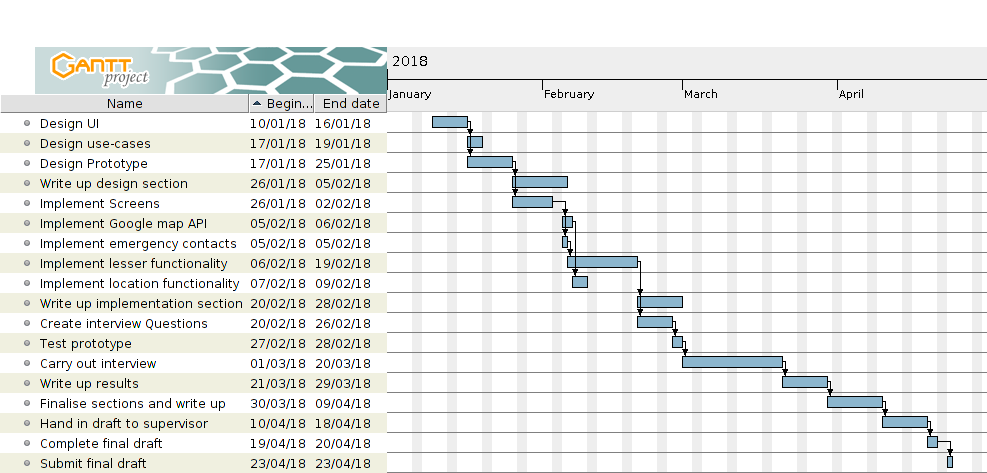
\includegraphics[width=200mm]{GanttChart.png}
\end{landscape}
\newpage
\section{Project Plan Writeup}
\label{sec:ProjectPlanWriteup}
\begin{center}
	\begin{longtable} {|c|c|c|p{60mm}|}
		\hline
		Task & Start Date & End Date & Description \\
		\hline 
		Design user interface & 10/01/2018 & 16/01/2018 & To design the user interface of the application, which is integral to the project. The UI needs to be clear and all functionality should be easily activated. \\
		\hline
		Design use cases &  17/01/2018 & 19/01/2018 & To design use cases to make clear how actors interact with the system and how basic functionality is achieved.\\
		\hline 
		Design prototype & 17/01/2018 & 25/01/2018 & Designing the application, combining the UI design with functionality, ensuring everything is laid out well and is as easy as possible for the user to follow. \\
		\hline 
		Write up design section & 26/01/18 & 05/02/2018 & Write the design section of my dissertation once all of the design elements are finished, ensuring that it is still fresh and I am not rushing to do it later. \\
		\hline 
		Implement screens & 26/01/18 & 02/02/2017 & Implement the screens that were designed for the UI.\\
		\hline 
		Implement Google Map API & 05/02/2018 & 06/02/2018 & Integrate the Google Maps API to make the location/map aspect of the application easier to implement. \\
		\hline
		Implement emergency contacts & 05/02/2018 & 05/02/2018 & Integrate/allow users to add their emergency contacts either manually or through accessing the users contacts on their phone. \\
		\hline
		Implement lesser functionality & 06/02/2018 & 19/02/2018 & Implementing other functionality, such as panic button, fake call button, and alarm button. \\
		\hline
		Implement location functionality & 07/02/2018 & 09/02/2018 & Perhaps the most important part of the application, implementing the location parts of the application, such as sending updates to contacts of location, or displaying messages within a certain area through the social media platform. \\
		\hline 
		Write up implementation section & 20/02/2018 & 28/02/2018 & Write the implementation part of dissertation after implementing a complete prototype. \\
		\hline 
		Create interview questions & 20/02/2018 & 26/02/2018 & Create multiple questions to ask users during the interview, including a usability study, asking the user to complete tasks, and asking their opinion of the application. \\
		\hline 
		Test prototype & 27/02/2018 & 28/02/2018 & Doing the interview questions myself and ensuring the interview is acceptable. I will make sure the functionality works and then conduct a pilot study on one participant to ensure any unbiased interview questions are removed. \\
		\hline 
		Carry out interview & 01/03/2018 & 20/03/2018 & Carry out the interview with participants over a two week period, to ensure maximum participants. \\
		\hline 
		Write up results & 21/03/2018 & 29/03/2018 & Gather all answers to interview, correlate the results, and write them up. \\
		\hline
		Finalise sections and write them up & 30/03/2018 & 09/04/2018 & Add all the sections already written up to one document and make sure they relate to each other. \\
		\hline 
		Hand in draft to supervisor & 10/04/2014 & 18/04/2018 & Hand in first draft of dissertation to supervisor and wait for feedback. \\
		\hline 
		Complete final draft & 19/04/2018 & 20/04/2018 & Using supervisors feedback, refine dissertation and fix all mistakes. \\
		\hline 
		Submit final draft & 23/04/2018 & 23/04/2018 & Submit dissertation. \\
		\hline
	\end{longtable}
\end{center}
\newpage
\chapter{Professional, Ethical, Social, and Legal Issues}
\label{sec:PESL}
For this project, we must consider how this application will fit into the following categories:
\begin{itemize}
\item \textbf{Professional:} I am not anticipating any professional issues with this project. 
\item \textbf{Ethical:} While designing the study carried out in semester 1, ethical approval was difficult to obtain, due to the implications of personal safety. It was difficult to create a survey about personal safety without causing discomfort to those who may have been attacked or had an experience while walking around alone. It is also difficult to test whether or not an application would improve personal safety, as it would involve putting participants into unsafe and dangerous situations and seeing if the application is effective. However, as this is incredibly unethical, I am planning on just using hypothetical vague situations that do not reference anything explicitly. During the survey, all participants agreed to take part and were informed they had the right to exit the study whenever they liked.  
\item \textbf{Social:} In terms of social considerations, and based on the information in section \ref{sec:GenderDifference} of this dissertation, females are more likely to be using a personal safety application, and so this is a focus for the application. 
\item \textbf{Legal:} There are legal implications to this application also. For example, if the application is wrong and causes the user to panic, and phone the police, then it raises the matter of wasting police time. It would be recommended to the user to only contact emergency services when something has actually happened (followed by someone, etc.) and to contact family/friends if they are feeling unsafe. There would also be a disclaimer detailing this on the application. 
\end{itemize}
\newpage
\chapter{Project Design}
\label{sec:ProjectDesign}
\section{Use Cases}
\label{sec:UseCases}
\begin{figure}[h]
	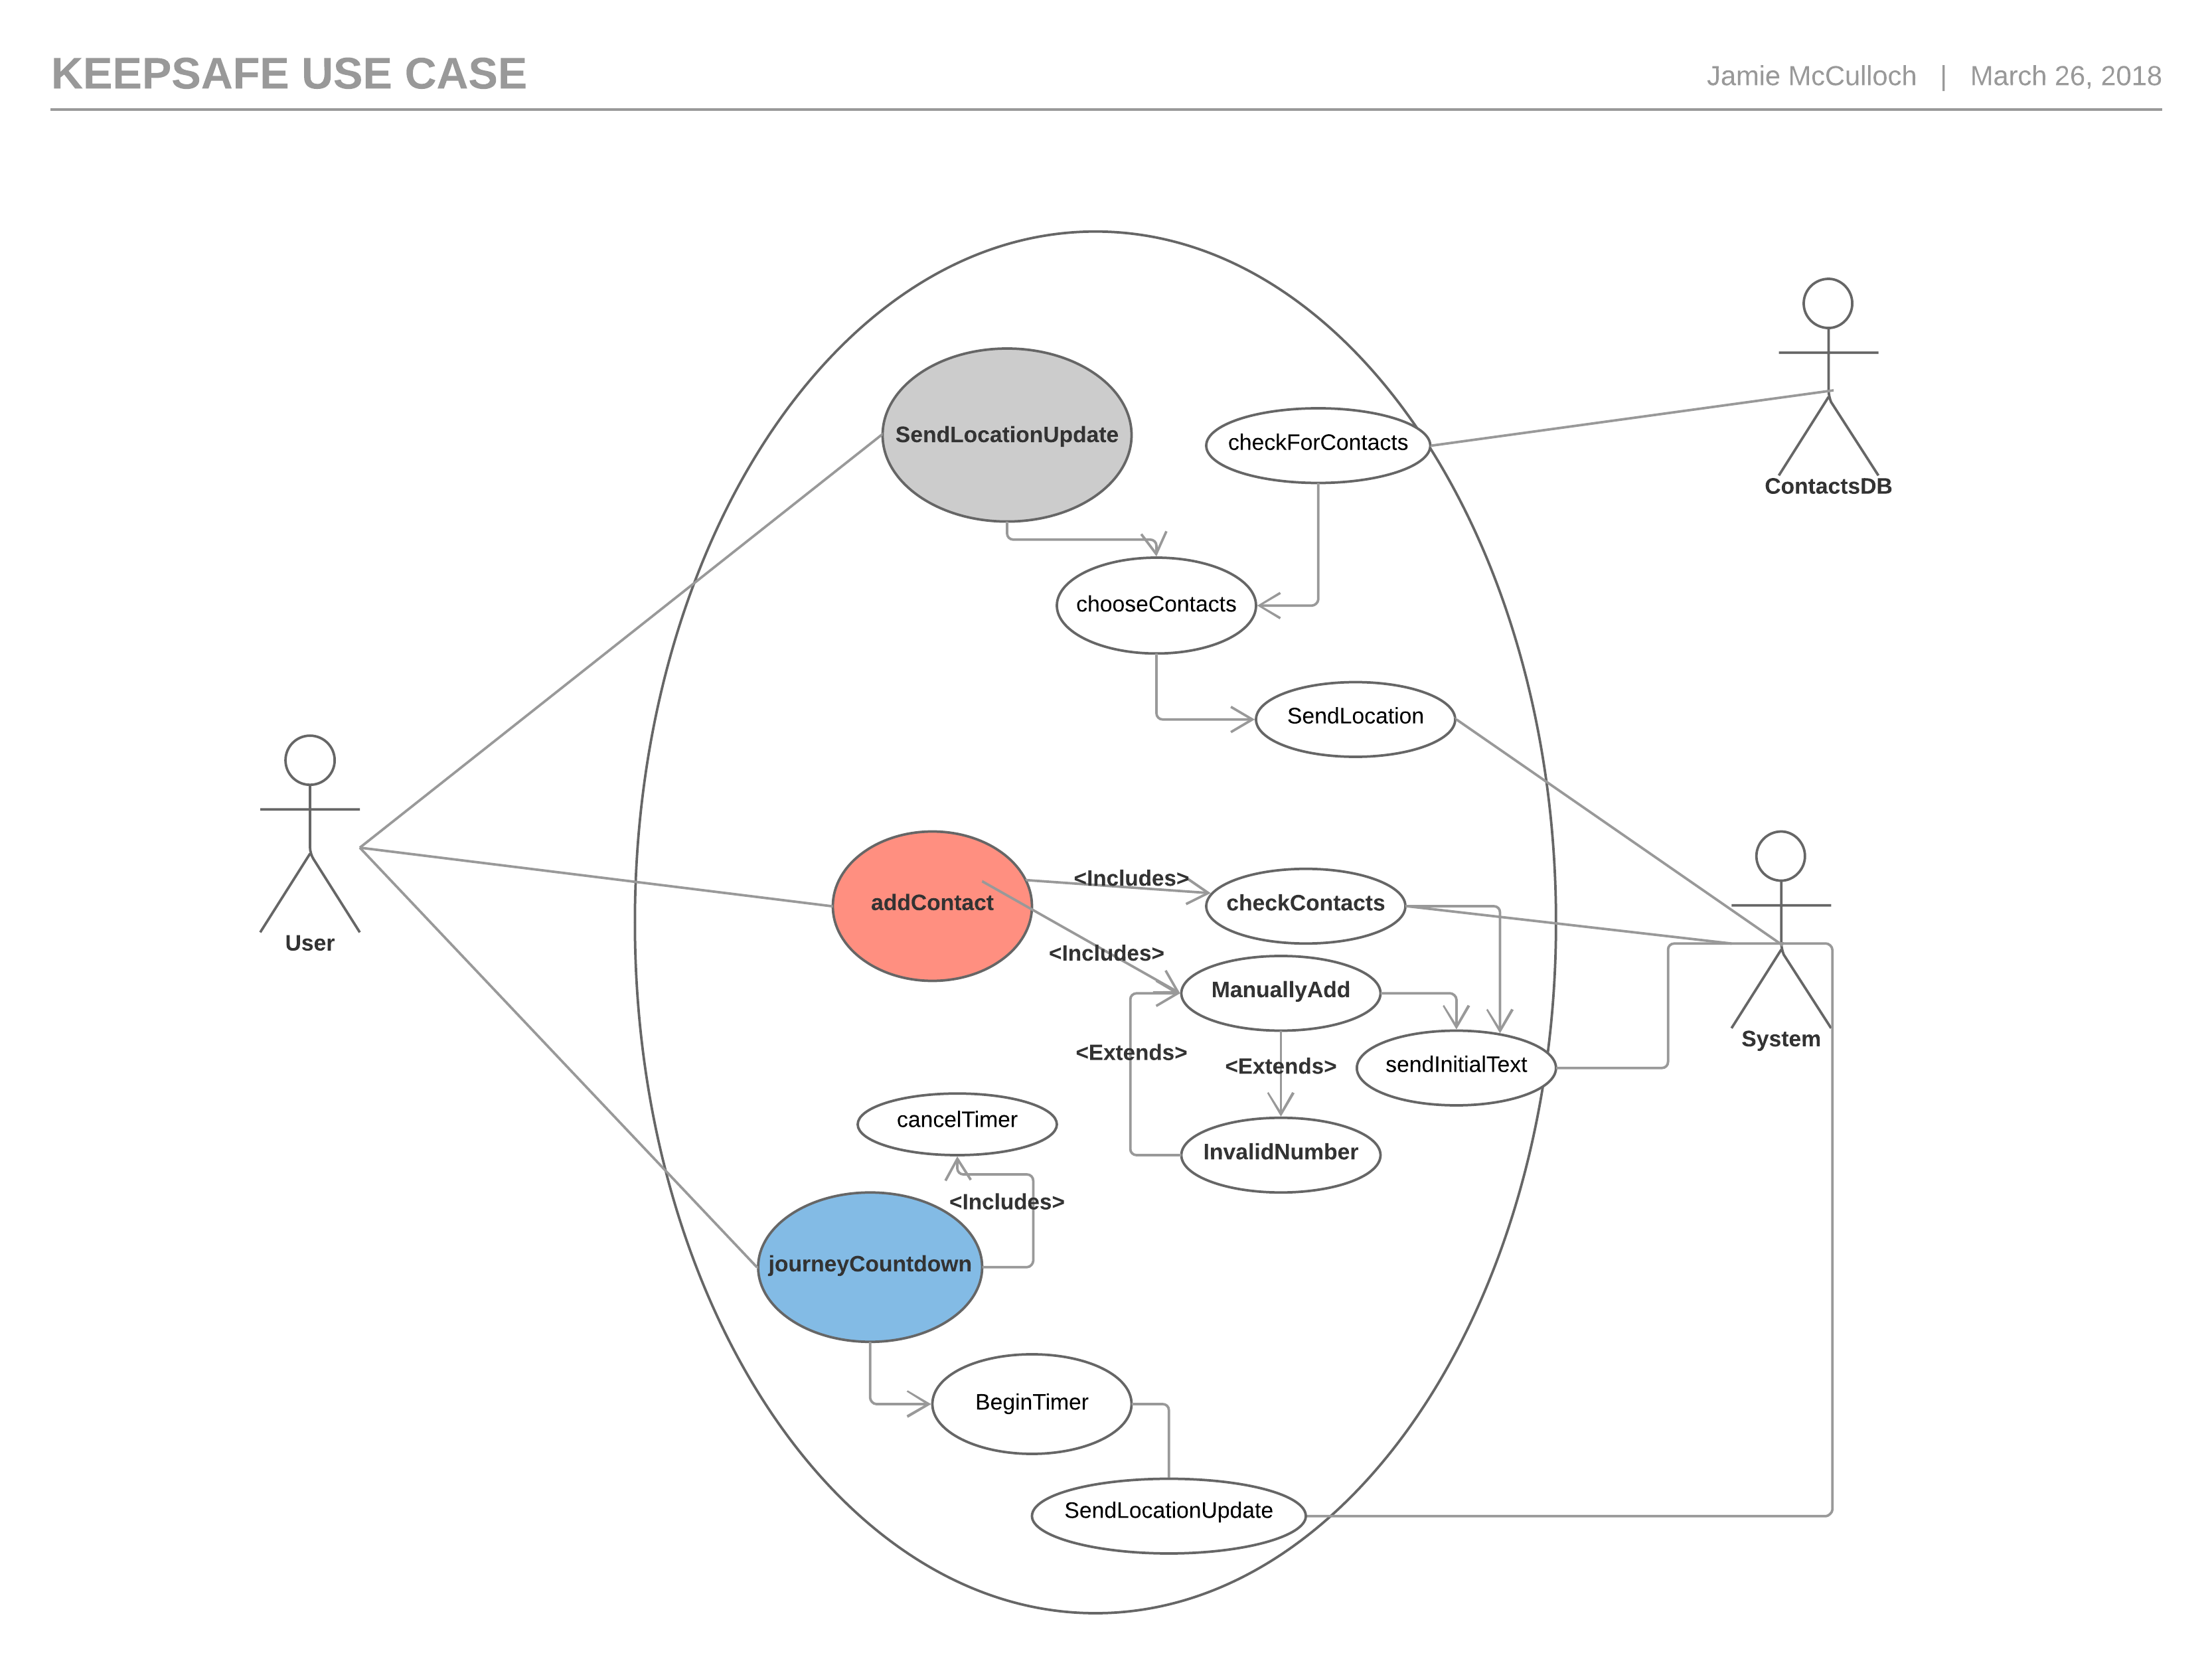
\includegraphics [width = 190mm]{KeepSafe.png}
	\caption{Use Case Diagram for KeepSafe}
	\label{fig:UseCase}
\end{figure}
I created one use case diagram, involving three of the most important features of the application - adding an emergency contact, sending a location update, and setting a journey countdown timer. I have also added use case textual descriptions, for both features implemented and future features. These are available in appendix C. 

\section{Initial User Interface and Name}
\label{sec:InitUI}
I decided before creating the application, that I would design the user interface (UI) first. This allowed me to gauge what functionality would appear on which screens. To create a UI, I used the online tool FluidUI \cite{fluidui}, which includes an Android template, with recognisable components. This allowed me to visualise exactly what the application would look like, and would highlight if a certain area of the activity (screen) was too cluttered, or if the buttons on the navbar were too close together. Another feature of FluidUI is that it can link activities  together if specified by the user. With this, I was able to check if an activity linked to another activity would work, and would suit the application. This was incredibly useful in deciding the original user interface design for the application, and gave me a good starting point to start development.
During this initial stage of design I also created a name for the application - KeepSafe. I feel like this perfectly encapsulates what the application should be doing and how it works - by keeping the user safe. Figure \ref{fig:InitialUIdesign} shows what the UI was initially intended to look like \\ 

\begin{figure}[h]
\centering
	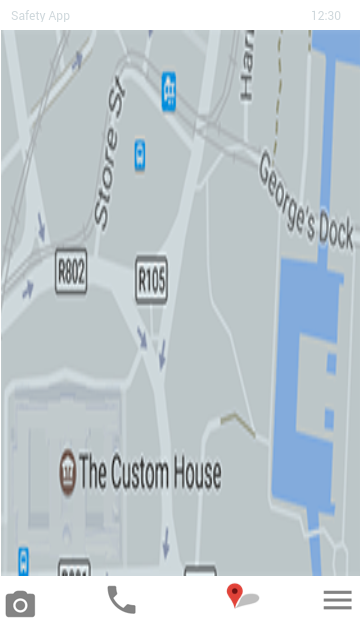
\includegraphics[width=3cm, height=6cm]{homepage}
	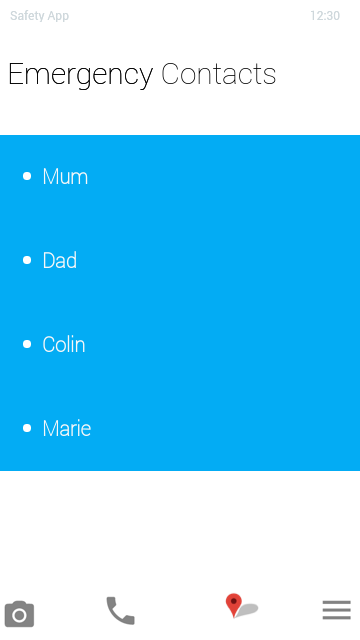
\includegraphics[width=3cm, height=6cm]{emergencycontacts}
	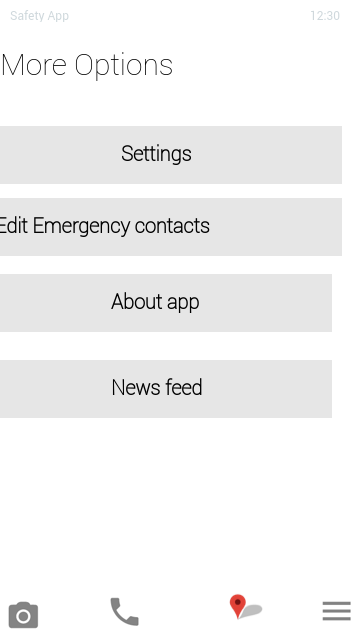
\includegraphics[width=3cm, height=6cm]{morepage}
	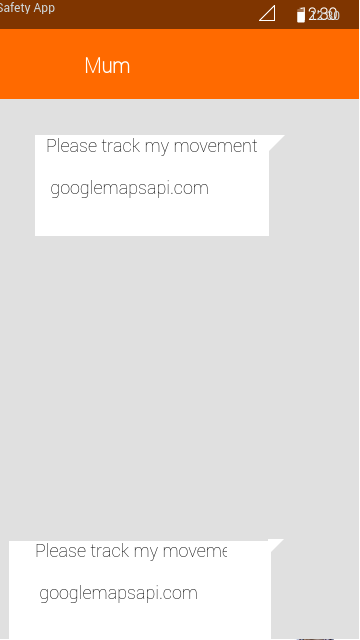
\includegraphics[width=3cm, height=6cm]{textpage}
		\caption{Initial UI design}
		\label{fig:InitialUIdesign}
\end{figure}
Figure \ref{fig:InitialUIdesign} shows four initial screens - a homepage, emergency contacts, a settings page, and the messaging screen (in this order). This was encapsulating all basic functionality that I aimed for. \\ \\
\textit{Homepage} - I intended on the application opening on the Google Maps screen, showing the users location and allowing them to view their surroundings. \\ \\
\textit{Emergency Contacts} - This screen would display the users stored emergency contacts, and allow them to call from within this activity. It would also allow the user to add/delete contacts as they like. \\ \\
\textit{Settings} - This page would allow the user to change the settings within the application, as it was to be fully customisable. It would also link to activities that were not as important to be on the navigation bar (that runs along the bottom of all screens). \\ \\
\textit{Messaging} - This screen would call the user's phones native messaging application, and populate the contacts with who is in the user's emergency contacts, and set the text to be a link to Google Maps with the user's latitude and longitude, allowing a pinpoint for the users location on the map.
\chapter{Implementation}
\label{sec:Imp}
Throughout this project, I implemented three prototypes, the first differing drastically from the latter two. Below I will detail each stage, and the functionality for each version. 
\section{Intended functionality}
\label{sec:IntendedFunc}
Through using the results from my initial survey (see section \ref{sec:FunctionalReq}), I found what functionality the majority of users would like, with the most popular being the ability to send location updates (82\%), a panic button (74\%) and an alarm sound being played at users request (53\%). With this in mind, I gradually built this functionality up over three prototypes. This allowed me to focus on getting each part working well before moving on to the next. However this was not all the application was intended to do, a significant advantage of KeepSafe is the ability to store emergency contacts within the application - meaning the user does not need to know phone 
numbers off the top of their head, and it makes it far easier to add contacts. I intended on importing the contacts from the phone to the application, and then allowing the user to click on them from within the application, this would link to a SQLite database and store the contacts name and number. There will also be an option to manually enter the name and number if the user prefers. \\
\\Taking inspiration from other personal safety applications - like bSafe\cite{bSafe} and SafetiPin\cite{safetipin} - I also intended on linking the camera application on the user's phone to allow for video recording/picture taking. This also doubled as having an audio recorder (as the video would record audio also). This would help reassure the user that if they were concerned about something/someone, they could have easy access to their camera to record and document what was happening. The application would allow the user to save the file to their phones internal storage and access at a future time. \\ Another feature I intended to make available within my application is a journey countdown timer. This would allow the user to enter a time in the application that they are allocating for their journey (for example 20 minutes). Once this timer has reached zero, the application will send out a location update to all emergency contacts stored within the application. To me, this was a very important feature, if the user is unable to access their phone, or they are in trouble during their walk, then the update will send automatically and hopefully help the user as their emergency contacts will know their location upon the countdown ending. \\\\Lastly having a link to Google Maps API would allow users to see their location on a map from within KeepSafe. I intended on this being used moreso if the user is in a location they are unfamiliar with, and may need some guidance as to how to find their way to their location. This would allow the user to quickly be taken to Google Maps to use their route planner feature. This was originally going to be the homepage to the application, however through multiple iterations this ended up being changed.  
\\I also decided that the program I would be using to create, compile, and run the application was Android Studio \cite{androidstudio}, which is the official integrated development platform for Android. This made the whole process of developing the application simpler, as there are a lot of resources online for Android Studio, and as it is the official platform, a lot of questions surrounding it are answered online and easily available. 
\section{Prototype 1} 
\label{sec:Prototype1}
\subsection{Implementing Prototype 1}
\label{sec:ImpPrototype1}
The first prototype created for KeepSafe followed the initial design laid out in section \ref{sec:InitUI} of this report. The application opened up displaying the Google Map API, which also showed the users current location in the form of a red marker on the screen. Along the bottom of the application was a navigation bar, similar to the one shown in Figure \ref{fig:InitialUIdesign} of section \ref{sec:InitUI}. This linked to the native messaging application on the phone, with the text field being populated with a link to Google Maps (this approach also allows those who do not have the Google Maps application on their phone to open it on their browser).
In terms of extracting the user's location using the phones GPS, I imported the LocationManager class from Android, and set up a variable that would call this class, and request the GPS longitude and latitude, the code below in figure \ref{fig:locationUpdate} is an extract of getting the users location: 
\begin{figure}[H]	
	\singlespacing
	\begin{lstlisting}
	\\RequestLocation.java
	
	LocationManager locationManager = (LocationManager) getSystemService(Context.LOCATION_SERVICE);
	
	locationManager.requestLocationUpdates(
		LocationManager.GPS_PROVIDER,
		MINIMUM_TIME_BETWEEN_UPDATES,
		MINIMUM_DISTANCE_CHANGE_FOR_UPDATES,
		new myLocationListener()
	);
	
	
	\end{lstlisting}
	\caption{Code to extract users location}
	\label{fig:locationUpdate}
\end{figure}
To then put this data into a format suitable to be sent to an emergency contact, I use the locationManager variable set up in figure \ref{fig:locationUpdate}, to extract the longitude and latitude, and then put this into a Google Map link. In figure \ref{fig:messageLocation}, this is done and added to a text message to be sent to a contact, which will be impemented in Prototype 2.\\
\begin{figure}[H]
\singlespacing
	\begin{lstlisting}
	Location location = locationManager.getLastKnownLocation(LocationManager.GPS_PROVIDER);
	
	
	if (location != null) {
	String message = "A MESSAGE FROM KEEPSAFE: \n You can track " + userName + "'s location here: http://maps.google.com/maps?q=loc:" + String.format("%f,%f", location.getLatitude(), location.getLongitude());
	}
	\end{lstlisting}
	\caption{Excerpt showing how the location update is created}
		\label{fig:messageLocation}
\end{figure}
Another button on the navigation bar was to a camera, which would open the users camera application on their phone and allow them to take a picture. This picture was then stored on their phone storage within their gallery. This feature was intended to be used in case the user found something/someone suspicious, they could take a photo from within the application for convenience instead of exiting and opening their camera. The last button on the navigation bar linked to settings, which was just a placeholder for future functionality. \\
\\ Importantly, the first prototype was simply to ensure that the location update worked, as this is fundamentally the most important feature to the app. Based on the study I conducted in section 3.1, 82\% claimed the most important feature was the location tracker/updater. This process involved linking the Google Map API to the application, I done this by linking the API to my Gmail account, and then using the key generated by Google to link to my application. From this I added permissions to the Android Manifest file (which "describes essential information about your app to the Android build tools, the Android operating system, and Google Play." \cite{manifest}). The following permissions were added to ensure the application had access to the phone's current location:   \\
\begin{figure}[H]
	\singlespacing
\begin{lstlisting}
	android:name="android.permission.ACCESS\_FINE\_LOCATION"
	android:name="android.hardware.location.gps"
\end{lstlisting}
\caption{Location Permissions}
\label{fig:LocPer}
\end{figure}
As a sidenote, the FINE\_LOCATION could be changed to COARSE\_LOCATION but I went with FINE as I wanted the location to be as accurate as possible. I had some issues regarding allowing the location to be read in by the application, but by changing the SDK version from 16 to 22 in the Gradle file of Android Studio. The Gradle file details to Android Studio how to compile and build the application to run on Android. I was able to run the application and see my location, and also to extract the longitude and latitude of the GPS coordinates and to concatenate them with a web URL for Google Maps. \\\\
The camera also linked with the application by using: \\
\begin{figure}{H}
	\singlespacing
\begin{lstlisting}
	android:name="android.permission.CAMERA"
\end{lstlisting}
\caption{Camera Permission} 
\label{fig:CameraPer}
\end{figure}
and allowed the user to take a picture from within the application and save it to their phones internal storage. \\

\subsection{Evaluation of Prototype 1}
\label{sec:EvalPrototype1}
Apart from this however no other functionality was added to prototype 1, and the application looked rather basic. After some deliberation I realised that the application did not have to open up on the Maps activity, and in fact, a lot of users may not even use this part of the application. The main crux of the project was to send location updates, and this should have been at the forefront of the development. Another drawback to Protoype 1 is the lack of emergency contacts. This feature was not developed until Protoype 2, and thus the user had no option to save contacts within the application. This resulted in the user having to type in their contacts name from within the messaging application, which was not ideal as it meant spending extra time, when it was crucial that the application worked in as few clicks as possible. \\ The navigation bar that was to be displayed consistently on every screen was not implemented in Prototype 1, buttons were used in a horizontal Linear Layout to emulate a navigation bar but I knew this was not going to be a permanent solution.
With all of this in mind, a lot was changed between Prototype 1 and Prototype 2, which is detailed in section 7.3.
\section{Prototype 2}
\label{sec:Prototype2}
\subsection{Implementing Prototype 2}
\label{sec:ImpPrototype2}
The main focus of prototype 2 was to allow the user to store emergency contacts within the application, create a panic button, and to maintain a consistent layout within the full application, using a navigation bar. In terms of the emergency contacts, I decided on accessing the users contacts stored on their phone, and store them in the application to print out. This was achieved through adding the: \\
\begin{figure}{H}
	\singlespacing
\begin{lstlisting}
	android:name="android.permission.READ\_CONTACTS"
\end{lstlisting}
\caption{Reading Contacts Permission}
\label{fig:readContacts}
\end{figure}
 permission. My plan was to link this to a database, which would store the name and number of the contact selected by the user. To do this, I created a SQLite Database, within the project. I called the database Contacts, and had multiple query functions within the helper class which allowed me to extract information from the database to use within the application. For example, when a contact was clicked from the users stored contacts, an alert dialog would appear, asking if the user would like to add this contact as an emergency contact. If the user selected \textit{yes} then the insert function was called with the suitable parameters. The contact was then stored in the Contacts database which consisted of three columns - ID (the primary key), ContactName (the contacts name), and ContactNo (the contacts phone number). This was a simple solution and did not store any unnecessary data. To delete an emergency contact, the user types in the name of the contact. 
\\If the user does not want to add a contact through their saved contacts, they also had the option of adding manually, which took the user to a form with name and number fields. To then send a location update to these stored contacts, I added the following code to the \textbf{RequestLocation.class}, continuing on from figure \ref{fig:messageLocation} in section \ref{sec:ImpPrototype2}.\\ 
\begin{figure}[H] 
	\singlespacing
	\begin{lstlisting} 
SmsManager.getDefault().sendTextMessage(textContacts, null, message, null, null);
}
\end{lstlisting}
\caption{using the SMS manager to send the location update} 
\label{fig:textLocation}
\end{figure}
Within the same method as defined in figure \ref{fig:messageLocation}, figure \ref{fig:textLocation} shows the extra line of code that calls the phones SmsManager, and sends an update. The variable \textit{textContacts} is a String array that stores all of the numbers of emergency contacts. The user can modify if they want to send a location update to everyone in their emergency contacts, or if they want to modify who they send it to. Figure \ref{fig:textLocation} shows the former, as this will send a text to everyone in \textit{textContacts} immediately. 
\\Within Prototype 2, I also created a navigation bar, created out of Radio Buttons, which allowed the user to seemlessly navigate through the application. The navigation bar was stored in a \textbf{MainActivity.java} which each other activity extended from. The advantage to this was that it meant if a new button was added, it would only be changing one class, and any new activities would only need to extend this class to also be consistent in layout, and contain a navigation bar. \\A panic button was deemed an important feature to a personal safety application by 74\% of the participants of the study I carried out (see section \ref{sec:SurveyResults}). The problem with the implementation of this was simply - what would the panic button do? It would perhaps change from user to user, and more importantly from situation to situation. Sometimes the user may favour using the panic button to call emergency services, but may also prefer it if the panic button played a blaring alarm noise to deter a criminal. To solve this, I created an option in the Settings page of the application to allow the user to pick what they wanted the panic button to do. For this implementation these were: 
\begin{itemize}
	\item Call emergency services (999)
	\item Record video 
	\item Send location update
	\item Play alarm sound
\end{itemize}
These were implemented as radio buttons, and the user could select any option.\\
More functionality was added during development of Prototype 2, with the Settings page allowing the user to customise what certain buttons do. For example, the user could set the location updates to send to all stored emergency contacts without bringing up the message interface, or they could edit who the update would be sent to within the messaging interface. I also added a name variable to the application during this stage of development. This was to allow a name to appear on outgoing messages from KeepSafe. The theory behind this choice is that not everyone is saved under recognisable names on phones, and it also makes it easier to know exactly who is messaging you their location. \\ All of the selected settings were stored using Shared Preferences on the phone. Shared Preferences are key-value pairs, saved in an XML file and are private to the application. This allowed me to save "panic button settings" to be one option, for example "call 999". This would overwrite the previous value attributed with "panic button settings" and would save it with "call 999" instead. A case statement within the \textbf{MainActivity.java} was used to determine what to do with each situation. This also means more options can be added in future implementations if needed.  
An excerpt of code for this purpose is below in figure \ref{fig:panicSettings}:\\
\begin{figure}[H]
\singlespacing
\begin{lstlisting}
\\MainActivity.java

 SharedPreferences prefs = getSharedPreferences("Settings", MODE_PRIVATE);
 checkPanicSettings = prefs.getString("checkPanicSettings", "missing");

 switch (checkPanicSettings) {
 case "phone":
		 Intent callIntent = new Intent(Intent.ACTION_CALL);
		 callIntent.setData(Uri.parse("tel:999"));
		 startActivity(callIntent);
		 break;
 case "sendLoc":
		 Intent in;
		 in = new Intent(getBaseContext(), RequestLocation.class);
		 startActivity(in);
		 break;
\end{lstlisting}
\caption{Code for checking which panic button option is selected and executing}
	\label{fig:panicSettings}
\end{figure} 
The above code details an excerpt of the openPanic() method, which checked the corresponding pair to "checkPanicSettings" and determined which case statement should be used. 
Using SharedPreferences was vital, as it allowed all settings to be saved easily and retrieved quickly. It was also not suitable to put the panic button settings in a database, as it would be complicated to extract the correct setting and apply it to a case statement. \\\\
During developing Prototype 2, I decided upon adding states to the application, starting with 2 - standard and alert. These would be quick to change, and would result in the application changing behaviour. For example, in alert mode, a location update would be sent to everyone in the emergency contacts, without being able to be edited, regardless of the settings chosen by the user. Any future update would also be sent to everyone, with no messaging interface appearing. There is also a countdown timer in alert mode, which when the user enters a time (in seconds) the application counts down and sends a location update once the timer expires. This feature would be useful when the user is concerned about something on their walk, and decides to update their emergency contacts every 30 seconds (for example). \\\\
The interface for alert mode is different also. The top notification bar changes to blue, and there is no navigation bar. This allows the user to clearly determine which mode they are in. From within alert mode, the user can also easily phone the emergency services, or record video from within the application. As part of the usability study I conducted in semester 2, participants are asked what their opinion of this feature is, and whether any features are missing from the list of buttons in alert mode. \textbf{ADD QUICK RESULTS HERE}. \\
 
\subsection{Evaluation of Prototype 2}
\label{sec:EvalPrototype2}
Prototype 2 was the basic application which would allow the user to store emergency contacts, send location updates, change states, use a panic button, and record video. I would take this further within Prototype 3 and focus more on usability over functionality.
This prototype also contained a consistent layout among all screens, and allowed the user to seemlessly traverse the application without difficulty. A few challenges were encountered when trying to make the navigation bar work. The main challenge stemmed from Android Studio\cite{androidstudio}. When creating a new activity within Android Studio, it prompts you for a template - if the bottom navigation bar template is selected then fragments need to be used to swap what is being displayed on the main activity, and not a new activity for each. Upon first implementing this, I realised that each time the bottom navigation bar was opening a new activity, it was opening the "Home" section of the bar, regardless of which activity. This caused a lot of issues as it resulted in a lot of code duplication, and it was very difficult to send data through the application and store it. Upon realising this, I instead implemented a horizontal radio button bar at the top of the main activity, and extended this to all other activities resulting in a quick, consistent layout. It also resulted in a lot less code duplication and the ability to store data in a central place (either Shared Preferences or a database). \\\\
Another challenge I faced during implementing Prototype 2 was which kind of database to use. Within Android development there are multiple different types of database system, each with their own advantages and disadvantages. The type I went for was an SQLite database. From previous experience, I am very familiar with SQL-like systems, specifically MySQL, and the fact that the queries written in SQLite are very similar to those of MySQL meant I could pick them up easily and quickly. I created a helper function which held all queries for the database, and called them depending on what I needed within the appliciation. 

\section{Prototype 3} 
\label{sec:Prototype3}
\subsection{Implementation of Prototype 3} 
\label{sec:ImpPrototype3}
As discussed in section \ref{sec:Prototype2}, Prototype 2 had the majority of basic functionality and could be a standalone product. However I still had some lesser functionality to implement - such as a journey countdown displayed on the homepage, the application recognising it had not been opened before and asking the user for an initial setup, implementing a \textit{name} variable to allow the application to be more personal, among other things. First off however, I had to ensure that the user had their location enabled on their phone. Without this the application would fail to send location updates, and other than some basic functionality, would not work correctly. To counter this, I created a function to be called each time the application is opened to check if the location is enabled. If it was not, an alert dialog would appear and explain this to the user, if the user agreed, the location would be enabled from within the application. This was a quick and easy way to ensure the application would work as intended and also meant the user did not have to leave the application to enable location.\\  As mentioned in section \ref{sec:Prototype2}, the settings page within the application allowed the user to customise what they wanted certain functions to do, for example - change what the panic button does, or if the user wanted to send the location update to everyone instantly. If these values are not set then the application will not recognise what to do and will crash. By creating a boolean \textit{isFirstTime}, I was able to determine if the application had run before, if it had not, then \textbf{SettingsFirstTime.java} would be run instead of \textbf{Homepage.java}. This would then allow the user to set up the application, by entering their name, to initially set up what the panic button does when clicked, and to choose if they want the location updates to send to everyone without confirmation or to bring up the messaging interface. If any of these settings are not initially set up, the user cannot start the application. There is also a reminder to add emergency contacts (however this is not forced as it is not required). 
\\\\Another feature I added during developing Prototype 3 was to send an automated message to an emergency contact when added, stating that they have been added as an emergency contact by the users name, for example: \\\\
\textit{You have been added as an emergency contact by Jamie through KeepSafe, expect some location updates!} \\\\
This message lets the contact know that they are chosen to be an emergency contact and that they should expect some updates. It is a simple feature but i feel like it adds a lot to the application, and it means the contact may be more likely to be checking their phone for updates. 
\subsection{Evaluation of Prototype 3}
\label{sec:EvalPrototype3}
With this being the final implementation of KeepSafe for this project, I feel it was successful. The changes from Prototype 2 to Prototype 3 were more improvements to the usability of the application instead of functionality. The purpose of this prototype was to make the application more appealing to the user, and to highlight the functionality behind the application to the user in a fluid, intuitive manner. The process of this prototype was to take what had already been implemented in terms of functionality and think how to improve it. For example - adding a first time settings page means that all variables within the Shared Preference key values had a corresponding value from initial start up. This kind of addition means the application is more robust and reliable - it does not crash on startup if the user has not first visited the settings page. Within the usabilty study I carried out in section \ref{sec:Usability} of this report, I queried if some of these additions were helpful, and received feedback from users based on this. 
\chapter{Components of KeepSafe}
\label{sec:Components}
In this section I will detail all of the activities and backend files for the project, what they are and for the activites screenshots of the layout. 
\section{Front End Components}
	\begin{tabular} {|c|p{125mm}|}
		\hline
		Component Name & Description\\
		\hline 
		aboutPage & A simple activity displaying information about KeepSafe, and what permissions it uses. \\
		\hline
		addContacts & A form allowing the user to manually enter a contact's name and number to be added to emergency contact.\\
		\hline
		alertPage & The \textbf{Alert} interface, containing a much simpler UI and implementing a quick countdown feature to send a location update in \textit{x} amount of seconds.\\
		\hline
		emergContacts & The activity which shows the saved contacts within the application, and allows the user to add/delete contacts.\\
		\hline
		home & This is the initial activity, a contains a personal message to the user, and a journey countdown timer (in minutes). \\
		\hline
		mainActivity & Arguably the most important class, this is the root activity, all other activities extend this. It specifies the navigation bar and also sets the panic button's and alert button's location.\\
		\hline
		mapsActivity & Extends the GoogleMaps API and displays a map, with the users location specified with a red marker. \\
		\hline
		removeContact & Allows the user to delete a contact by entering the contact name.
	\\ \hline
		requestLocation & Finds the longitude and latitude of the user and sends it to emergency contacts in whatever way the user has specified. \\
		\hline 
		settings & A form with radio buttons, allowing the user to specify what the want certain features to do - panic button, and how they would like to send a location update. Also allows user to change the \textbf{alert} mode.
		\\ \hline
		settingsFirstTime & A form that only opens on the first open from the user, and allows them to set initial settings, thus giving initial values to everything. 
		\\ \hline 
		showAllContacts & Populates a list view with all of the users contacts stored on their phone, on click the contact gets added to the emergency contacts of the application. \\
		\hline
	\end{tabular}
	\section{Back End Components} 
	\begin{tabular} 	{|c|p{125mm}|}
		\hline
		Component Name & Description \\
		\hline 
		ContactsDB & This class specifies the database, and the columns in it. It is used to get parameters of the database. \\
		\hline
		myDBHandler & Contains functions used to create, delete, and modify the database. Also query functions to extract contact name and number. Extends SQLiteOpenHelper. \\
		\hline
		myLocationListener & Extends LocationListener, as a constructor class to set up a locationManager. \\
		\hline
	\end{tabular}
	\\
	Although there is not much to the backend, in terms of the application, these are crucial. To store the contacts name and number, I set up an SQLite Database, with three columns - a unique ID, a contact name, and a contact number. I then linked this with the \textit{emergContacts} class, allowing the user to add contacts into the database through either manually entering the name and number (through \textit{addContact}) or through the phones already stored contacts (through \textit{showAllContacts}). Then when the user would like to send a location update, they have the option to send it to all contacts, or edit the contacts they wish to send it to. To do this, I have created a String array, containing the number of all contacts, then I send specify this array as the 'recipient' of the text message. If the contacts name is stored in the phone, the name will automatically show up, through the phones internal storage recognising it. I utilise another array to show all emergency contacts, through using a ListView in XML, and displaying a new String array that contains both name and number of each contact. This is shown below in figure \ref{fig:showEmergContacts}\\
	\begin{figure}[H]
		\centering
	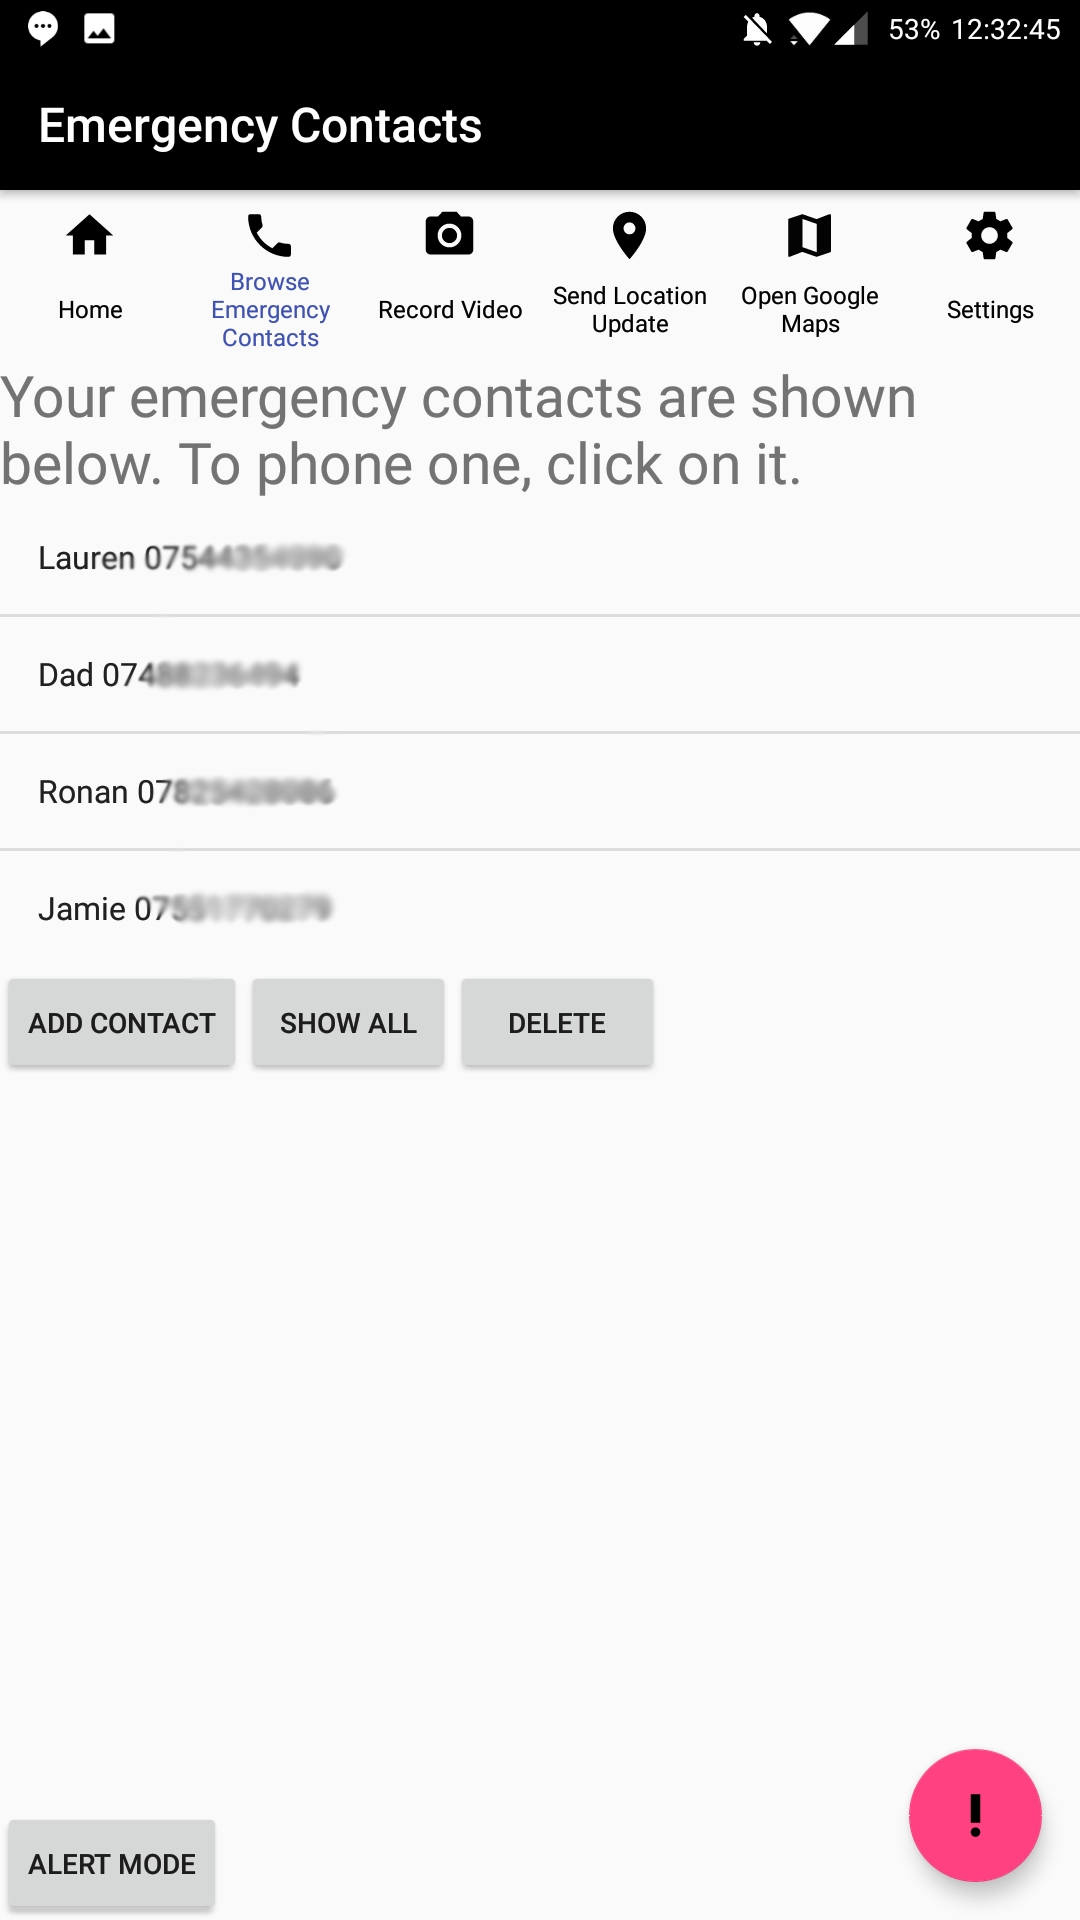
\includegraphics[width=6cm, height=9.5cm]{emergContactsSafe}
	\caption{Showing users emergency contacts}
	\label{fig:emergContacts}
	\end{figure}
	
	\chapter{Future Plans} 
\label{sec:FuturePlans}
Despite the application implementing the majority of key features that were requested from the initial survey, and from my experience with other applications, there were still some that I was not able to implement. 
\section{Time Filters}
\label{sec:TimeFilters}
If I were to continue developing KeepSafe, I would implement some form of time filter - for example, if the user accesses the application from a certain time. Based on my initial survey (found in Appendix B) I found between 6pm and 6am was the most common time to feel unsafe, with 77\% of participants agreeing to this. Using this, I would implement a time filter, in which if the user opens up the app during these 12 hours (or hours set specifically by the user) then the application would open in the \textbf{Alert Mode}, as this is the quicker of the two interfaces to interact with. The time filter range would be customisable, as is the rest of the application, allowing the user to specify what time range they would like this to apply to, they can also disable the feature if need be. This feature is not available on the two personal safety applications I tested, bSafe\cite{bSafe} and SafetiPin, \cite{safetipin} and I feel as though it would add a unique selling point to KeepSafe. Unfortunately, I did not have the time to implement this feature, as I encountered challenges during the applications development that caused my schedule to be delayed, these are described in evaluation sections of each prototype (section \ref{sec:EvalPrototype1}, \ref{sec:EvalPrototype2}, \ref{sec:EvalPrototype3}). 
\section{Proximity Based Social-Media}
\label{sec:ProxSocialMedia}
During the initial study I undertook to gather requirements and people's reaction to a personal safety application, I offered an option to implement a proximity based social media platform. This would allow users of KeepSafe to let other users know what was happening around them, even if they did not have direct contact with them. My initial thoughts on this would be, KeepSafe would display messages uploaded to an SQLite database, containing the author of the post and the message, along with the location at which the message was posted (using the same longitude and latitude extraction function as the main application). I would then implement a display function that, if the user was within a certain range of the post, it would display. This would be done by creating a radius around the longitude and latitude of where the message was posted, and then only displaying the message to other users when they are within that radius. The idea behind this is that users can help each other, and report things that they may not deem noteworthy enough to tell the emergency services. For example, if they notice a certain person always hanging out while they are walking, they could post it on this platform to let others know to watch out for them. This would be another unique point, as the two application I tested, bSafe and SafetiPin, did not have this feature or anything related to it. 
\chapter{Testing} 
\label{sec:Testing} 
I carried out multiple methods of testing during the development of KeepSafe, as detaied below. This helped me keep a track of issues annd fix them quickly.
\section{Unit Testing} 
Unit testing is the testing of individual components or functions, to ensure they work in \textbf{isolation}. I used this method to test every function I wrote, I used print statements to test that functions were working. For example, I printed out the longitude and latitude relative to the users current location. By doing this, it allowed me to quickly check if there was any problems with the functions I was implementing, and fix them if necessary. This kind of testing was essential to me during development. 
\section{Component Testing} 
Component testing is normally carried out after unit testing, to test multiple 'units' together, and ensure they work with each other. For example, I tested that on adding an emergency contact to the database, that it would also send a text to the new contact informing them of this. All of the functionality could exist, however if it does not link together correctly it can become useless and a major bug to the system. Thus, it is important to find this out as soon as possible so it can be fixed quickly. 
\section{Usability Testing} 
Usability testing is ensuring the application is usable. That the layout is satisfactory, and nothing is obscured or overlapping. I carried out initial usability tests, making sure the application ran well and all components of the application ran and were easily readable. After judging the user interface to be acceptable, I conducted a usability study to gather the opinion of others, who had not seen the application before. This gave a useful insight into how usable the application was to a range of people - from students to senior citizens. It allowed for me to see if the user interface could be improved. The conclusions of the usability study are available in section \ref{sec:Usability}. 

\chapter{Usability study} 
\label{sec:Usability}
I conducted a usability study to test KeepSafe, both for functionality and for usability. I have carried out personal testing (see section \ref{sec:InitialTesting}) to ensure the functionality is there, and the application is robust, however my intention was that the participants would test the app thoroughly and would think of things I had not, allowing me to fix any major bugs. More importantly though, I wanted to find out if the application had a good user interface, and all users would be able to easily navigate the application. As I was familiar with the application (having created it), it was important for me to get other opinions on the interface, and ensure it was successful. I conducted interviews, lasting about 20 minutes, with participants and asked them to conduct certain tasks within the application. These ranged from adding an emergency contact, to sending a location update, to changing the settings (full set of questions in Appendix C). This allowed me to see if the interface was easy to navigate, and if the users would know what to do given a certain task. After each task, I also asked the participant their opinion on each task, on the application design, and if they would find the feature useful. 
\newpage
\bibliography{ref} 
\bibliographystyle{unsrt}
\newpage
\appendix
\chapter{Survey Questions}
\label{app:Survey}

1. What is your age, in years? \\
2. What gender do you identify with? \\
	- Male\\
	- Female \\
	- Rather not say\\
3. Have you ever felt unsafe while walking alone outside? \\
- Yes\\
- No\\
4. Is there a particular time of day that you might feel less safe while walking alone outside?\\
	- 12am-6am\\
	- 6am-12pm\\
	- 12pm-6pm\\
	- 6pm-12am\\
	- None, I don't think I feel unsafe at any particular time\\
5. Which of the following situations would make you feel unsafe while walking alone outside?\\
- Walking through a busy shopping centre\\
- Walking past a pub at midnight\\
- Walking through an unlit residential area\
- Hearing loud shouting behind you\\
- Walking to the supermarket during the day\\
- Walking without your phone\\
- None, I don't think I feel unsafe in any particular situation\\
- Other\\ \\ \\
6. Have you ever used a mobile phone to make you feel safer while walking alone outside?\\
- Yes\\
- No\\
7. Have you ever used a ‘personal safety application’ to make you feel safer while walking outside alone?\\
-No\\
-Yes (please specify what app below)\\
8. In your opinion, what is the 3 most important features for a personal safety app?\\
(If you wouldn’t find a personal safety application useful, you only need to select the one choice.)\\
- Location tracker\\
- Alarm sound (plays loud alarm when activated)\\
- Panic button (calls emergency contacts instantly)\\
- Alternate route planner to avoid unsafe areas\\
- Selfie mode\\
- Fake incoming call button\\
- None, I don't think I would find a 'personal safety app' useful\\
- Other\\
9. Would you be comfortable with your location being tracked as part of a ‘personal safety application’?\\
- Yes, all the time\\
- Yes, as long as I could turn it off\\
- Not at all\\
\newpage
\chapter{Survey Results} `	
\label{app:Results}
\bigskip
1. \begin{tabular} {|c|c|}
	\hline
		Age Range & Count \\
		\hline
		16-25 & 35 \\
		\hline
		26-36 & 5 \\
		\hline
		36-45 & 5 \\
		\hline
		46-55 & 11 \\
		\hline
		56+ & 18 \\
		\hline
	\end{tabular}
\bigskip

2. \begin{tabular} {|c|c|}
	\hline
	Gender & Count \\
	\hline
	Male & 26 \\
	\hline
	Female & 48 \\
	\hline
\end{tabular}
\bigskip

3. \begin{tabular} {|c|c|}
	\hline
	Felt Unsafe? & Count \\
	\hline
	Yes & 61 \\
	\hline
	No & 13 \\
	\hline
\end{tabular}
\bigskip

4. \begin{tabular} {|c|c|}
	\hline
	Unsafe Time? & Count \\
	\hline
	 12am-6am & 27 \\
	 \hline 
	 6am-12pm & 3 \\
	 \hline
	 12pm-6pm & 5 \\
	 \hline
	 6pm-12am & 30 \\
	 \hline
	 None, I don't think I feel unsafe at any particular time & 9 \\
	\hline
\end{tabular}
\bigskip

5. \begin{tabular} {|c|c|}
	\hline
	Unsafe Situation? & Count \\
	\hline
	Walking through a busy shopping centre & 1 \\
	\hline
	Walking past a pub at midnight & 29 \\
	\hline
	Walking through an unlit residential area & 52 \\
	\hline 
	Hearing loud shouting behind you & 50\\
	\hline
	Walking to the supermarket during the day & 0 \\
	\hline
	Walking without your phone & 20 \\
	\hline
	None, I don't think I feel unsafe in any particular situation & 4 \\
	\hline
	Other & 3 \\
	\hline
\end{tabular}
\bigskip 

6. 
\begin{tabular} {|c|c|}
	\hline
	Mobile phone to make you feel safer? & Count \\
	\hline
	Yes & 52 \\
	\hline
	No & 22 \\
	\hline
\end{tabular}
\bigskip 

7. \begin{tabular} {|c|c|}
	\hline
	Mobile app to make you feel safer? & Count \\
	\hline
	Yes & 2* \\
	\hline
	No & 72 \\
	\hline
\end{tabular}\\
*Both answers are disregarded as misunderstood question and answer does not apply. 
\bigskip 

8. \begin{tabular}{|c|c|}
		\hline
		Most important feature (pick 3) & Count\\
		\hline
		Location Tracker/Updates & 61 \\
		\hline
		Panic Button & 55 \\
		\hline
		Alarm Sound & 39 \\
		\hline
		Fake Incoming Call & 30 \\ 
		\hline
		Alternate Route Planner & 15 \\
		\hline
		None & 3 \\
		\hline
		Selfie Mode & 0 \\
		\hline
	\end{tabular}
	\bigskip 
	
9. 	\begin{tabular}{|c|c|}
	\hline
	Comfortable with location tracking? & Count\\
	\hline
	Yes, all the time & 15 \\
	\hline
	Yes, if I could turn it off & 55 \\
	\hline
	Not at all & 4 \\
	\hline
\end{tabular}
\chapter{Use Cases}
\section{SendLocation}
\textbf{Name:} sendLocation \\
\textbf{Description:} Send users location coordinates to an emergency contact \\
\textbf{Actors} User, Contact\\
\textbf{Preconditions:}
\begin{itemize}
	\item Phone location is enabled
	\item Contact is stored in application as an emergency contact
	\item Map button on UI is clicked on
\end{itemize}
\textbf{Basic Flow:} 
\begin{itemize}
	\item System derives location from gps
	\item User selects a contact to send it to
	\item System sends text message with coordinates to contact
\end{itemize}
\textbf{Alternate Flows:}
\begin{itemize}
	\item User cancels the request
	\item Application returns to homescreen 
\end{itemize}
\textbf{2.}
\begin{itemize}
	\item Contact is not stored in app
	\item User adds contact
	\item System derives location from gps
	\item User selects a contact to send it to
	\item System sends text message with coordinates to contact
\end{itemize}
\textbf{Exceptional Flows:} \\
\textbf{1.}
\begin{itemize}
	\item Location is not enabled
	\item Prompt user to turn on location permissions
\end{itemize}
\textbf{2.} 
\begin{itemize}
	\item User has no signal on phone 
	\item Message sends when user gets signal again
\end{itemize}
\textbf{Postconditions:}
\begin{itemize}
	\item User has sent a location update through the application
\end{itemize}

\section{addContact}
\textbf{Name:} addContact\\
\textbf{Description:} Add an emergency contact to the app\\
\textbf{Actors:} User, System\\
\textbf{Preconditions:} 
\begin{itemize}
	\item User selects the add emergency contacts button
\end{itemize}
\textbf{Basic Flow:}
\begin{itemize}
	\item User enters name for the contact
	\item User enters a valid (11 digit) number
	\item System accepts contact and adds to emergency contact list
\end{itemize}
\textbf{Alternate Flows:} 
\begin{itemize}
	\item User selects ‘import contact’
	\item The system accesses the phones contacts
	\item User selects contact they want to add
\end{itemize}
\textbf{Exceptional Flows:} \begin{itemize}
	\item User does not enter a valid number for contact
	\item System prompts user to fix this or return to home screen
\end{itemize}
\textbf{Postconditions:}
\begin{itemize}
	\item The system has added contact to the emergency contact list
\end{itemize}





\textbf{Name:} firstOpen \\
\textbf{Description:} What happens when the application is opened for the first time \\
\textbf{Actors:} User, System\\
\textbf{Preconditions:}\\
User has not opened up the application before \\
\textbf{Basic Flow:} \\
The system will prompt user to pick privacy options \\
The system will prompt user to select what screen they would like to open on \\
The system shall ask user to customise the bottom screen \\
The system shall give a short tutorial on how to use application\\
\textbf{Alternate Flows:} \\
\textbf{Exceptional Flows:}\\
\textbf{Postconditions:}\\
The user has successfully customised the app to users liking \\


\textbf{Name:} setJourneyCountdown \\
\textbf{Description:} User sets a countdown, once expired the system will send a location update\\
\textbf{Actors:} User, System\\
\textbf{Preconditions:} \\
\textbf{Basic Flow:}\\
The user shall specify a time to countdown from (in minutes)\\ 
The system shall begin a countdown \\
Once the timer has expired, the system shall send a location update to all emergency contacts \\
\textbf{Alternate Flows:}\\
The user cancels the countdown during it \\
\textbf{Exceptional Flows:}\\
The user enters an invalid time \\
The system notifies the user\\
\textbf{Postconditions:}\\
A journey countdown has been set \\





\textbf{Name:} PanicButton\\
\textbf{Description:} Activation of panic button\\ 
\textbf{Actors: User, System}\\
\textbf{Preconditions:}\\
Panic Button is selected\\
\textbf{Basic Flow:} \\
The system will check to see what panic button option is selected in settings\\
The system will carry out the appropriate response\\
\textbf{Alternate Flows:}\\
\textbf{Exceptional Flows:}\\
\textbf{Postconditions:}\\
The panic button will be executed \\



\textbf{Name:} accessingSocialMedia\\
\textbf{Description:} Accessing the social media portion of the app\\
\textbf{Actors:} User, System, messageDB\\
\textbf{Preconditions:}\\
User has location turned on \\
User selects social media option in app\\
\textbf{Basic Flow:} \\
The system will set up a proximity and collect messages that were given within this proximity based on their location in the messages database\\
The system will display these messages\\
\textbf{Alternate Flows:}\\
\textbf{Exceptional Flows:} \\
The user’s location is unknown \\
The system will alert user and prompt them to turn on location\\
\textbf{Postconditions:}\\
Social media segment will be running\\



\textbf{Name:} PostComment\\
\textbf{Description:} Post a comment on a social media segment\\
\textbf{Actors:} User, System, MessageDB\\
\textbf{Preconditions:}\\
Location is turned on \\
Social media segment is open\\
\textbf{Basic Flow:} \\
The system shall allow user to compose a message\\
The user shall input their message\\
The system shall save their message into a database, with the message, the author, and the location it was posted at\\
\textbf{Alternate Flows:}\\
\textbf{1.}\\
The system shall allow user to compose message \\
The user submits an empty message\\
The system will prompt user to enter characters in message\\
\textbf{2.}\\
The system shall allow user to compose message \\
The user quits the app halfway through\\
The system saves the message to drafts \\
User can go in and find message in drafts and upload it\\
\textbf{Exceptional Flows:}\\
\textbf{Postconditions:}\\
The user will have successfully added a message to the media board\\

\end{document}
